\documentclass[preprint,12pt]{elsarticle}

\usepackage{xeCJK} % Support Chinese characters

\setCJKmainfont{BiauKai}[Path = ./fonts/chinese/ , Extension = .ttf , ]

\journal{Knowledge-Based Systems}

\begin{document}

\begin{frontmatter}

\title{Lightweight Chinese News Summarization via Knowledge Distillation and Curriculum Learning}

\author[1]{Yu-Hao Wang}
\ead{f74116152@gs.ncku.edu.tw}

\author[1]{Shang-Liang Chen\corref{cor1}}
\ead{slchen@mail.ncku.edu.tw}

\cortext[cor1]{Corresponding author.}

\affiliation[1]{
    organization={Department of Computer Science and Information Engineering, National Cheng Kung University},
    addressline={No. 1, University Road},
    city={Tainan},
    postcode={701},
    country={Taiwan}
}

%% Abstract
\begin{abstract}
In today’s era of information overload, readers often lack time to engage with full news articles and may be misled by sensational headlines. This work presents a lightweight Chinese news summarization model designed for resource-limited devices while maintaining strong comprehension and fluency. By combining knowledge distillation with a five-stage curriculum, covering traditional Chinese conversion, aspect extraction, reasoning construction, and summary generation, the model achieves efficient parameter compression without sacrificing quality. We further evaluate data generation methods and training strategies, including staged learning-rate adjustment, selective parameter freezing, and LoRA adaptation. Experiments show that resetting the learning rate in the final stage enhances optimization stability, while full-parameter fine-tuning remains the most effective strategy. Contrary to expectations, LoRA and partial freezing offer minimal efficiency gains. The trained 0.5B-parameter model matches or surpasses larger counterparts, generalizes well to unseen datasets, and effectively eliminates structural and formatting errors inherited from the teacher. These results demonstrate the viability of compact yet high-quality summarization models suitable for practical mobile deployment.
\end{abstract}

%%Research highlights
\begin{highlights}
\item Introduces a \textbf{five-stage curriculum learning framework} tailored for compact LLMs.
\item Combines \textbf{knowledge distillation} with progressive training to improve fluency.
\item Proposes a \textbf{summary-first data generation} strategy that yields coherent and focused training samples.
% \item Shows that \textbf{resetting the learning rate in the final stage} improves optimization stability and end-stage refinement.
\item Achieves \textbf{3B-tier summarization quality} with a \textbf{0.5B-parameter model}.
\item Corrects \textbf{teacher-induced structural and formatting errors}, improving Traditional Chinese summary quality.
\end{highlights}

%% Keywords
\begin{keyword}
chinese news summarization \sep lightweight models \sep knowledge distillation \sep curriculum learning
\end{keyword}

\end{frontmatter}

%% main text
%%
\section{Introduction}

In today’s fast-paced society, readers often lack the time to thoroughly engage with complete news articles. Sensational headlines and fragmented information can easily distort public understanding. A compact Chinese summarization model capable of running on mobile devices can address this issue by delivering concise, meaningful summaries, thereby improving both the efficiency and quality of information acquisition.

This research aims to integrate knowledge distillation and curriculum training strategies to compress model parameters while enhancing generalization and language comprehension. The ultimate objective is to develop and deploy a high-quality Chinese news summarization system on mobile devices—achieving a balance between compactness and performance.


\section{Methodology}

\subsection{Data Collection}
To build the training corpus, a custom web crawler was developed to collect news articles from \textit{United Daily News}. Additionally, the YeungNLP/firefly-pretrain-dataset was incorporated as supplementary pretraining data. This combination provided both domain-specific news coverage and a broad linguistic foundation for model training.

\subsection{Model Selection}
Two models from the Qwen2.5 family were adopted \cite{qwen2.5}, both based on the Transformer architecture \cite{vaswani2017}. The student model, Qwen2.5-0.5B-Instruct, is a lightweight 0.5-billion-parameter model optimized for efficient fine-tuning and deployment. The teacher model, Qwen2.5-32B-Instruct, was used for generating synthetic data, providing reasoning guidance, and offering evaluation signals during experiments.

\subsection{Curriculum Training}
Training was structured into five progressive stages (S1–S5) designed to gradually increase task complexity. First, traditional Chinese text was standardized using OpenCC (S1). Next, essential aspects were extracted from each article (S2), followed by the construction of semantic triples that captured relationships among those aspects (S3), inspired by TriSum \cite{trisum}. Building on this foundation, the model generated summaries conditioned on the article content and the extracted aspects/triples (S4). Finally, the model was trained to produce summaries directly from raw news content (S5), representing the most challenging stage.

\subsection{Data Generation Strategies}
Several strategies for generating training data were explored.  
The \textbf{V1} strategy generated aspects, triples, and summaries jointly in a single step.  
\textbf{V2} followed a sequential pipeline—first generating aspects, then triples, and finally summaries.  
\textbf{V3} reversed this process by generating the summary first and then inferring supporting aspects and triples.  
Finally, \textbf{V4} extended V3 with manual error correction to reduce noise and improve overall quality.

\subsection{Training Strategies}
We explored several fine-tuning strategies to identify the most effective setup for curriculum training.  
The baseline employed a standard decaying learning-rate schedule, gradually lowering the rate as training progressed from Stage 1 to Stage 5.  
However, this monotonic decay risked premature convergence in later, more complex stages.  
To address this, the variant \texttt{lr\_adj} retained the decay pattern in Stages 1–4 but reset the starting learning rate in Stage 5 to match the initial value of Stage 1.  
This adjustment provided a renewed optimization signal at the final, most demanding stage, while still allowing intra-stage decay to stabilize learning.  

We also examined selective parameter freezing to analyze the contribution of specific network components:  
\texttt{only\_attn} froze all parameters except attention layers, and \texttt{only\_mlp} froze all parameters except MLP layers.  
Additionally, LoRA-based adaptation \cite{lora} was applied to both MLP (rank 160) and attention (rank 32) layers, introducing low-rank trainable matrices to reduce the number of fine-tuned parameters.  
Combinations of these strategies were further explored to identify potential synergies.

\subsection{Evaluation Metrics}
Model outputs were evaluated using both automatic and teacher-aligned metrics. ROUGE-1, ROUGE-2, and ROUGE-L measured lexical n-gram overlap with reference summaries, while BERTScore \cite{DBLP:journals/corr/abs-1904-09675} captured semantic similarity.
In addition, the teacher model (32B) acted as a judge to evaluate naturalness and information coverage, providing a complementary qualitative evaluation to automatic metrics.

\section{Experiments}

\subsection{Comparison of Data Generation Strategies}
The first experiment evaluated how different data generation strategies affected downstream summarization.  
Direct reasoning (V1), which required the teacher to infer aspects and triples before summarization, produced incomplete and incoherent outputs.  
Although some logical consistency remained, the generated summaries lacked comprehensive content coverage, reducing their usefulness for training.

The stepwise approach (V2) aimed to mitigate this issue by decomposing generation into multiple stages. However, this actually worsened coherence, producing “out-of-focus” results in which key elements deviated from the final summary. This suggests that excessive decomposition may amplify inconsistencies instead of reducing them.

In contrast, the summary-first strategy (V3) showed clear advantages. By first generating a coherent summary and then deriving supporting aspects and triples, it achieved the highest scores across all evaluation metrics (ROUGE, BERTScore, and Judge).  
The manually corrected V4 variant further improved data quality, establishing it as the preferred strategy.

\begin{table}[t]
\centering
\begin{tabular}{lccccc}
\hline
Model & R-1 & B-F1 & Judge & R-2 & R-L \\
\hline
4stg\_v3 & \textbf{45.5} & \textbf{77.9} & \textbf{70.3} & \textbf{24.3} & \textbf{37.6} \\
4stg\_v1 & 43.8 & 76.8 & 64.0 & 22.1 & 35.5 \\
4stg\_v2 & 37.6 & 69.4 & 65.1 & 17.5 & 23.4 \\
\hline
\end{tabular}
\caption{Performance Comparison by Data Generation Strategy}\label{strategy_comparison}
\end{table}

\subsection{Training Strategy Comparison}
The second experiment compared the learning-rate schedules and parameter-freezing techniques described above.
The \texttt{lr\_adj} variant, which restored the Stage-5 starting learning rate to the initial value, achieved superior performance compared with a strictly decaying schedule.  
This suggests that small student models benefit from stronger optimization in the final stage, where summarization tasks are most complex.

Both \texttt{only\_attn} and \texttt{only\_mlp} configurations achieved competitive results, indicating that attention and MLP layers contribute comparably to summarization performance.  
For instance, the \texttt{only\_mlp} variant maintained a high BERTScore (78.6\%), demonstrating robust semantic alignment.

In contrast, LoRA adaptation did not improve results in this context—performance either plateaued or slightly declined.  
Overall, these findings highlight that full-parameter fine-tuning with a carefully staged learning-rate reset remains the most effective strategy for compact summarization models (see Table~\ref{training_strategy_comparison}).

\begin{table}[t]
\centering
\begin{tabular}{lccccc}
\hline
Model & R-1 & B-F1 & Judge & R-2 & R-L \\
\hline
4stg\_v3-lr\_adj & \textbf{48.4} & \textbf{79.3} & 72.8 & \textbf{25.7} & \textbf{40.1} \\
4stg\_v3-lr\_adj-only\_mlp & 46.6 & 78.6 & 71.5 & 24.2 & 38.4 \\
4stg\_v3-lr\_adj\_lora & 45.6 & 78.0 & \textbf{73.6} & 23.3 & 37.4 \\
4stg\_v3 & 45.5 & 77.9 & 70.3 & 24.3 & 37.6 \\
4stg\_v3-lr\_adj-only\_attn & 45.2 & 77.8 & 69.1 & 23.0 & 37.1 \\
\hline
\end{tabular}
\caption{Performance Comparison by Training Strategy}\label{training_strategy_comparison}
\end{table}

\subsection{Effect of Curriculum Stages}
The third experiment examined the impact of curriculum stage count.  
While single-stage setups occasionally achieved slightly higher ROUGE-1 scores, multi-stage training consistently produced better linguistic quality and output stability, especially in Traditional Chinese generation.

\begin{table}[t]
\centering
\begin{tabular}{lccccc}
\hline
Model & R-1 & B-F1 & Judge & R-2 & R-L \\
\hline
Qwen2.5-0.5B\_4stg\_v3 & 45.5 & \textbf{77.9} & \textbf{70.3} & \textbf{24.3} & 37.6 \\
Qwen2.5-0.5B\_1stg\_v3 & \textbf{45.9} & 77.9 & 68.8 & 23.7 & \textbf{37.7} \\
\hline
\end{tabular}
\caption{Performance of Different Stage Numbers with Decaying Learning Rate}\label{tab:stage_lr_decay}
\end{table}

\begin{table}[t]
\centering
\begin{tabular}{lccccc}
\hline
Model & R-1 & B-F1 & Judge & R-2 & R-L \\
\hline
Qwen2.5-0.5B\_1stg\_v4-lr\_adj & \textbf{47.0} & \textbf{78.8} & \textbf{75.9} & \textbf{24.5} & \textbf{38.9} \\
Qwen2.5-0.5B\_4stg\_v4-lr\_adj & 46.8 & 78.6 & 75.2 & 24.2 & 38.6 \\
Qwen2.5-0.5B\_5stg\_v4-lr\_adj & 46.5 & 78.6 & 75.1 & 23.9 & 38.3 \\
\hline
\end{tabular}
\caption{Performance of Different Stage Numbers without Decaying Learning Rate}\label{tab:stage_no_lr_decay}
\end{table}

\begin{figure}
\centering
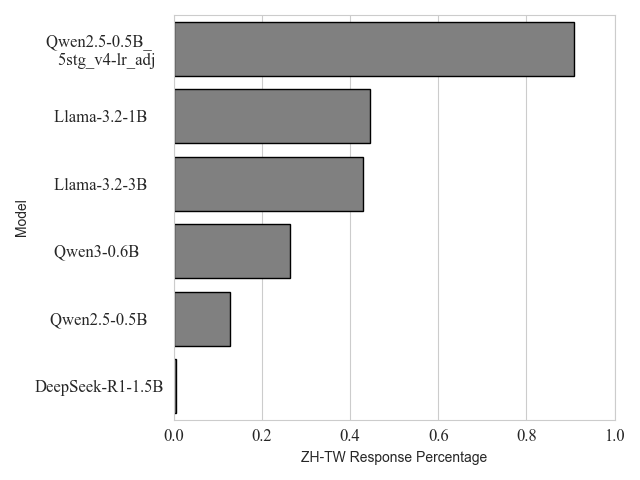
\includegraphics[width=\textwidth]{figures/zh_tw_result_percentage_overall.png}
\caption{Proportion of Traditional Chinese responses generated by each model. The proposed 0.5B model with 5-stage curriculum achieves the highest ratio, surpassing even 3B models.}\label{fig:zh_tw_result}
\end{figure}

Curriculum benefits were also found to depend on pretraining scale.  
When pretraining was extensive, the improvements were modest; however, with smaller pretraining datasets, curriculum learning provided substantial gains, helping compensate for weaker initial representations.

\begin{table}[t]
\caption{Performance of Custom Pretrained Models with Different Curriculum Stages}
\label{tab:custom_pretrain_stage_comparison}
\centering
\begin{tabular}{lccccc}
\hline
Model & R-1 & B-F1 & Judge & R-2 & R-L \\
\hline
Custom-pretrained-4stg\_v3-lr\_adj & \textbf{13.3} & \textbf{50.6} & \textbf{0.9} & \textbf{1.8} & 4.0 \\
Custom-pretrained-1stg\_v3-lr\_adj & 11.8 & 50.5 & 0.6 & 1.5 & \textbf{5.0} \\
\hline
\end{tabular}
\end{table}

\subsection{Generalization to Unseen Datasets}
To evaluate generalization, inspired by the work of \cite{basyal2023llms}, the trained model was tested on two unseen corpora: \textit{CLTS} \cite{clts} (long-form) and \textit{CNewSum(v2)} \cite{cnewsumv2} (headline-style).  
These datasets differ greatly from the training domain in style and topic diversity, providing a robust test of adaptability.  
Evaluation was conducted using ROUGE-1, ROUGE-2, and ROUGE-L metrics to measure cross-domain robustness.


\section{Results}

\subsection{Final Model Performance}
The final Qwen2.5-0.5B model achieved performance approaching that of 3B-scale models in all automatic metrics, marking significant improvements in abstraction and accuracy.  
It outperformed other small-scale models such as DeepSeek \cite{deepseek-r1}, Gemma \cite{gemma}, and LLaMA \cite{llama3}, with ROUGE-1 gains of 7–11\%.  
Compared with its pre-trained baseline, the post-trained model’s Judge score improved by 0.16, confirming notable gains in naturalness, informativeness, and abstractive capability.

\begin{table}[t]
\caption{Performance Comparison of Final 0.5B Model with Other Models of Similar Parameter Scale}
\label{tab:final_05B_comparison}
\centering
\begin{tabular}{lccccc}
\hline
Model & R-1 & B-F1 & Judge & R-2 & R-L \\
\hline
Qwen2.5-32B & \textbf{55.6} & \textbf{82.2} & 81.7 & \textbf{34.9} & \textbf{48.2} \\
Qwen2.5-3B & 49.5 & 79.8 & \textbf{83.8} & 26.2 & 40.1 \\
Qwen2.5-0.5B\_5stg\_v4-lr\_adj & 46.5 & 78.6 & 75.1 & 23.9 & 38.3 \\
Llama-3.2-3B & 43.3 & 76.8 & 74.3 & 20.7 & 34.7 \\
Gemma-3-1B & 41.8 & 76.0 & 72.6 & 18.3 & 31.2 \\
Qwen2.5-0.5B & 39.7 & 74.8 & 58.7 & 18.5 & 30.9 \\
Gemma-2-2B & 39.3 & 71.9 & 83.4 & 18.3 & 26.2 \\
Llama-3.2-1B & 38.7 & 74.1 & 63.4 & 16.9 & 29.5 \\
DeepSeek-R1-1.5B & 32.2 & 71.3 & 65.8 & 12.0 & 21.4 \\
\hline
\end{tabular}
\end{table}

\subsection{Traditional Chinese Generation}
In addition to overall performance, the model demonstrates marked improvements in linguistic handling. After post-training, the proportion of Traditional Chinese output rises significantly, even exceeding that of the teacher model. The percentage of responses completely free of Simplified Chinese characters is also higher than in other models, highlighting the effectiveness of the training data and curriculum strategy in producing culturally and linguistically appropriate text.

Beyond accuracy, the model showed substantial improvement in linguistic alignment.  
After post-training, the proportion of Traditional Chinese outputs rose markedly—surpassing even the teacher model.  
The share of responses entirely free of Simplified Chinese characters also increased, demonstrating that the curriculum design effectively enhanced cultural and linguistic fidelity.

\subsection{Generalization to Unseen Datasets}
The trained 0.5B model generalized well to unseen datasets, consistently outperforming its untrained baseline and approaching 3B-tier models in all ROUGE metrics on both \textit{CLTS} and \textit{CNewSum(v2)} (Table~\ref{unseen_datasets_simple}).  
Although not surpassing the 32B teacher, its proximity to 3B performance highlights strong abstraction and factual alignment despite its compact size.

These results confirm that the proposed curriculum and fine-tuning strategies enable compact models to achieve an effective trade-off between efficiency and generalization, acquiring meaningful semantic representations rather than relying on memorization.

\begin{table}[t]
\centering
\caption{
\textbf{Generalization Performance on Unseen Datasets (\textit{CLTS} and \textit{CNewSum(v2)}).}
Models are evaluated using ROUGE-1 (R-1), ROUGE-2 (R-2), and ROUGE-L (R-L) scores.
The two highest scores in each column are shown in \textbf{bold}.
Qwen2.5-32B achieves the best performance on CLTS, while Qwen2.5-3B slightly surpasses it on CNewSum(v2), demonstrating stronger domain adaptability.
The proposed multi-stage trained student (Qwen2.5-0.5B\_5stg\_v4-lr\_adj) maintains competitive generalization despite its smaller scale.
}
\label{unseen_datasets_simple}
\renewcommand{\arraystretch}{1.0}
\resizebox{\textwidth}{!}{
\begin{tabular}{lccc@{\hskip 15pt}ccc}
\hline
& \multicolumn{3}{c}{\textbf{CLTS}} & \multicolumn{3}{c}{\textbf{CNewSum(v2)}} \\
\cline{1-7}
\textbf{Model} & R-1 & R-2 & R-L & R-1 & R-2 & R-L \\
\hline
Qwen2.5-32B & \textbf{25.31} & \textbf{14.62} & \textbf{24.92} & \textbf{19.64} & \textbf{4.94} & \textbf{19.13} \\
Qwen2.5-3B & \textbf{22.36} & \textbf{10.96} & \textbf{21.63} & \textbf{20.09} & \textbf{5.15} & \textbf{19.61} \\ 
Qwen2.5-0.5B\_5stg\_v4-lr\_adj & 20.50 & 9.63 & 19.89 & 17.64 & 4.21 & 17.19 \\
Qwen2.5-0.5B & 18.61 & 9.03 & 18.25 & 15.63 & 3.73 & 15.28 \\
Gemma-3-1B & 17.79 & 7.94 & 17.26 & 16.44 & 3.87 & 16.02 \\
Llama-3.2-3B & 17.10 & 7.62 & 16.69 & 16.36 & 3.81 & 16.02 \\
DeepSeek-R1-1.5B & 16.45 & 8.63 & 15.96 & 11.10 & 2.51 & 10.72 \\
Llama-3.2-1B & 16.19 & 7.33 & 15.83 & 13.33 & 3.00 & 12.94 \\
Gemma-2-2B & 12.83 & 5.79 & 12.44 & 9.97 & 2.35 & 9.80 \\
\hline
\end{tabular}
}
\end{table}

\subsection{Mitigation of Teacher Model Errors}
Finally, the post-trained model effectively mitigated errors inherited from the teacher.
Among 30,296 samples, the teacher model produced 2,871 instances containing irregular endings or other apparent formatting errors (e.g., ``\texttt{\textbackslash n tworzyć \textbackslash n}''), excluding more complex issues such as imprecise phrasing or full-/half-width inconsistencies.
After training, the student model eliminated all such anomalies, confirming that staged curriculum learning and refined datasets successfully corrected structural and formatting artifacts present in the teacher outputs.


\section{Conclusion}
This study systematically explored strategies for developing a lightweight Chinese news summarization model, integrating data generation design, training configurations, and curriculum learning. The findings offer both methodological insight and practical guidance for achieving high-quality summarization under constrained computational resources.

In terms of data generation, the experiments revealed that direct reasoning and stage-by-stage decomposition tend to produce incomplete or unfocused outputs, limiting their utility as training data. By contrast, the summary-first approach consistently yielded coherent and comprehensive summaries, providing a stable foundation for downstream reasoning and facilitating more effective student–teacher distillation.

Regarding training strategies, applying a decaying learning rate across the early stages and restoring a stronger starting rate in the final stage (\texttt{lr\_adj}) yielded the best results. Combined with full-parameter fine-tuning, this approach outperformed LoRA-based and partial-freezing methods, showing that compact models benefit most from steady, end-stage optimization across all parameters. Moreover, contrary to expectations, LoRA and partial freezing provided little benefit in terms of training time or VRAM savings, reaffirming the practicality of full fine-tuning for small-scale summarization models.

The investigation of curriculum learning further emphasized its value, particularly under limited pretraining conditions. While multi-stage curricula produced modest improvements when large-scale pretraining was available, they substantially enhanced summarization accuracy, stylistic fidelity, and robustness for smaller, custom-pretrained models. This progressive task structure also enabled the student model to correct structural and linguistic imperfections inherited from the teacher model, such as irregular endings and formatting inconsistencies, demonstrating the corrective power of staged learning.

Evaluation on unseen datasets (\textit{CLTS} and \textit{CNewSum(v2)}) confirmed the generalization capability of the proposed approach. The trained 0.5B model consistently outperformed its untrained baseline and approached the performance of 3B-tier models across ROUGE and BERTScore metrics, showing strong abstraction and robustness despite its compact scale.

Collectively, these strategies produced a 0.5B-parameter model that achieves performance levels comparable to much larger models while maintaining superior efficiency and linguistic precision. Notably, the model surpasses even its teacher in Traditional Chinese generation quality, reflecting the success of the designed data and training pipeline.

In conclusion, this work demonstrates that through summary-first data generation, steady full-parameter fine-tuning, and staged curriculum progression, a compact model can achieve a balance between efficiency, robustness, and high-quality abstractive summarization. The proposed framework not only advances the practical deployment of summarization systems on mobile devices but also provides a scalable and reproducible path toward resource-efficient natural language processing.


\appendix
\section{Prompt Templates and Examples}
\label{app1}

This appendix provides the trained student model, the prompt templates and examples used in this study, including the complete prompt designs for final versions of essential aspect extraction, triple generation, summary generation, and model evaluation.
\newline

\noindent
\textbf{Published model:}\newline
{
  \footnotesize
  https://huggingface.co/BennyWang/Qwen2.5-0.5B-Instruct-Curriculum-5stage-v4-lr\_adj
}
\newline
\newline
\noindent
\textbf{Example news, essential aspects, triples, and summary (V3):}\newline
{
\small
\noindent
News:\newline
母愛不分物種。動保組織接獲民眾通報發現草叢有一窩胖嘟嘟奶汪,沒想到牠們的母親為了照顧這些孩子把自己餓成皮包骨,還有嚴重營養不良跟脫水狀況,對比起小狗們都肥碩健康,狗媽媽更是令人心疼。\newline
根據The Dodo報導,美國密蘇里州(Missouri)聖路易斯流浪動物救援組織(Stray Rescue of St. Louis,SRSL)日前接獲民眾通報,說草叢裡面發現一窩肥胖的奶汪,但卻找不到狗媽媽,希望他們可以派人來協助一下。動物救援組織工作人員湯姆森(Natalie Thomson)表示,當他們趕往民眾通報的現場,的確真的看到一窩被照顧得好好的奶汪,很像是被人飼養後遺棄在附近。\newline
但令動保人員意外的一幕出現了,他們過沒多久在附近的草叢找到了狗媽媽,可是這隻渾身骨瘦如柴、幾乎可以用皮包骨形容的黃狗顯然非常營養不良,跟牠一窩肥壯幼崽形成強烈對比,這隻狗媽媽顯得有些害怕人類,但牠並沒有逃跑或是圖保護孩子,反而是將目光投射在小狗身上,希望眼前的人類不要傷害牠的孩子。\newline
每一隻狗寶寶都相當健康可愛甚至還有點肥。 (圖/取自Stray Rescue of St. Louis官網)\newline
後來這一窩共10隻奶汪跟牠們孱弱的母親都被聖路易斯流浪動物救援組織帶回收容所,經過健康檢查後反而讓獸醫跟動保人員更難過了,因為這10隻小奶狗除了有點寄生蟲問題之外,沒有任何營養不良的狀況,甚至還有些過重,但狗媽媽卻嚴重營養不良還脫水,可以說為了照顧孩子鞠躬盡瘁。\newline
目前這一窩小奶汪都受到良好的照顧,不日將可開放認養,而狗媽媽則因為身體虛弱還需要靜養一段時間才可以考慮出養。湯姆森說,這隻狗媽媽其實是很溫柔的,只是個性比較慢熟,所以需要有愛心跟耐心的飼主陪伴,牠就會慢慢敞開心房願意相信人類。\newline
\newline
Summary:\newline
美國密蘇裡州一窩小狗被發現肥胖健康,但牠們的母親卻因照顧孩子而嚴重營養不良、脫水。這11隻狗已被救出,小狗們即將開放認養,母親則需繼續靜養。救援組織尋找有耐心的飼主,以陪伴這位溫柔但慢熟的母親。\newline
\newline
Essential aspects:\newline
[美國密蘇裡州]、[一窩小狗]、[肥胖健康]、[母親嚴重營養不良]、[脫水]、[已被救出]、[小狗們即將開放認養]、[母親需繼續靜養]、[救援組織尋找有耐心的飼主]、[溫柔但慢熟的母親]\newline
\newline
Triples:\newline
[美國密蘇裡州 | 發現 | 一窩小狗], [小狗 | 肥胖健康 | 狗媽媽], [狗媽媽 | 照顧孩子 | 嚴重營養不良], [狗媽媽 | 照顧孩子 | 脫水], [一窩小狗 | 被 | 救出], [小狗們 | 即將 | 開放認養], [狗媽媽 | 需 | 繼續靜養], [救援組織 | 尋找 | 有耐心的飼主], [狗媽媽 | 是 | 溫柔但慢熟的]\newline
\newline
}

\noindent
\textbf{Prompt for generating V3 summary:}\newline
{
\small
\noindent
System prompt:\newline
請根據以下新聞內容,為新聞生成一份100字內精簡的摘要,請用繁體中文回答。\newline
例如:\newline
生成摘要:\newline
% \newline
================================================\newline
% \newline
User prompt:\newline
新聞:\newline
\{news\}\newline
\newline
}

\noindent
\textbf{Prompt for generating V3 essential aspects and triples:}\newline
{
\small
\noindent
System prompt:\newline
請根據以下新聞內容以及摘要,提取新聞的關鍵要素與三元組,關鍵要素應為關鍵短句、名詞或事實,三元組應為[實體1 | 關係 | 實體2]的格式,這些三元組用於構成摘要,請用繁體中文回答。請將每個關鍵要素與三元組用[]與、分隔。例如:\newline
關鍵要素:\newline
[關鍵要素1]、[關鍵要素2]、[關鍵要素3]、...\newline
\newline
三元組:\newline
[實體1\_1 | 關係\_1 | 實體1\_2]、[實體2\_1 | 關係\_2 | 實體2\_2]、...\newline
% \newline
================================================\newline
% \newline
User prompt:\newline
新聞:\newline
\{news\}\newline
\noindent
摘要:\newline
\{summary\}\newline
\newline
}

\noindent
\textbf{Prompt for model scoring:}\newline
{
\small
\noindent
System prompt:\newline
你是一位語言評估專家。你的任務是根據文章與標準摘要,評估模型生成的摘要品質。\newline
請根據以下評分標準,從 0 到 20 為其打分:\newline
0:格式不正確或無意義的文字。\newline
1:完全無關,與文章毫不相干。\newline
2:虛構內容,語意不明。\newline
3:嚴重誤解,包含重大錯誤。\newline
4:幾乎無法反映原文,非常不完整。\newline
5:文法錯誤,缺乏連貫性與相關性。\newline
6:內容不完整且部分離題。\newline
7:遺漏關鍵要點,有輕微虛構。\newline
8:摘要過於模糊,缺乏具體性。\newline
9:簡潔,涵蓋大部分重點。\newline
10:可理解但可能遺漏細節。\newline
11:忠實但略有遺漏。\newline
12:大致正確但稍顯冗餘。\newline
13:準確、結構良好,但有輕微風格問題。\newline
14:涵蓋完整、清晰,語氣尚可改進。\newline
15:清楚、忠實且具風格。\newline
16:簡潔優雅,涵蓋所有重點。\newline
17:非常接近理想摘要,僅有些微瑕疵。\newline
18:優秀的摘要,易讀且內容完整。\newline
19:幾近完美,僅可做細微風格潤飾。\newline
20:完美——清楚、忠實、完整且優雅。\newline
請回傳"分數:"加一個整數分數(0–20),接著是一句簡短的理由(例如:「分數:17 —— 非常接近理想摘要,僅有些微瑕疵」)。\newline
% \newline
================================================\newline
% \newline
User prompt:\newline
文章:\newline
\{article\}\newline
\noindent
標準摘要:\newline
\{ground\_truth\}\newline
\noindent
模型生成摘要:\newline
\{response\}\newline
\newline
}


\begin{thebibliography}{11}

\bibitem{qwen2.5}
  Yang, A., Yang, B., Zhang, B., Hui, B., Zheng, B., Yu, B., Li, C., Liu, D., Huang, F., Wei, H., Lin, H., Yang, J., Tu, J., Zhang, J., Yang, J., Yang, J., Zhou, J., Lin, J., Dang, K., Lu, K., Bao, K., Yang, K., Yu, L., Li, M., Xue, M., Zhang, P., Zhu, Q., Men, R., Lin, R., Li, T., Tang, T., Xia, T., Ren, X., Ren, X., Fan, Y., Su, Y., Zhang, Y., Wan, Y., Liu, Y., Cui, Z., Zhang, Z., Qiu, Z.:
  Qwen2.5 Technical Report.
  arXiv preprint arXiv:2412.15115 (2024).
  https://doi.org/10.48550/arXiv.2412.15115

\bibitem{vaswani2017}
  Vaswani, A., Shazeer, N., Parmar, N., Uszkoreit, J., Jones, L., Gomez, A.N., Kaiser, Ł., Polosukhin, I.:
  Attention Is All You Need.
  In: Advances in Neural Information Processing Systems (NeurIPS), Vol. 30.
  Curran Associates, Inc. (2017).
  https://doi.org/10.48550/arXiv.1706.03762

\bibitem{trisum}
  Jiang, P., Xiao, C., Wang, Z., Bhatia, P., Sun, J., Han, J.:
  TriSum: Learning Summarization Ability from Large Language Models with Structured Rationale.
  In: Proceedings of the 2024 Conference of the North American Chapter of the Association for Computational Linguistics (NAACL),
   pp. 2805--2819. (2024).
  https://doi.org/10.48550/arXiv.2403.10351

\bibitem{lora}
  Hu, E.J., Shen, Y., Wallis, P., Allen-Zhu, Z., Li, Y., Wang, S., Wang, L., Chen, W.:
  LoRA: Low-Rank Adaptation of Large Language Models.
  arXiv preprint arXiv:2106.09685 (2021).
  https://doi.org/10.48550/arXiv.2106.09685

\bibitem{DBLP:journals/corr/abs-1904-09675}
  Zhang, T., Kishore, V., Wu, F., Weinberger, K.Q., Artzi, Y.:
  BERTScore: Evaluating Text Generation with BERT.
  In: International Conference on Learning Representations (ICLR). (2020).
  https://doi.org/10.48550/arXiv.1904.09675

\bibitem{deepseek-r1}
  DeepSeek-AI, Guo, D., Yang, D., Zhang, H., Song, J., Zhang, R., Xu, R., Zhu, Q., Ma, S., Wang, P., Bi, X., Zhang, X., Yu, X., Wu, Y., Wu, Z.F., Gou, Z., Shao, Z., Li, Z., Gao, Z., Liu, A., Xue, B., Wang, B., Wu, B., Feng, B., Lu, C., Zhao, C., Deng, C., Zhang, C., Ruan, C., Dai, D., Chen, D., Ji, D., Li, E., Lin, F., Dai, F., Luo, F., Hao, G., Chen, G., Li, G., Zhang, H., Bao, H., Xu, H., Wang, H., Ding, H., Xin, H., Gao, H., Qu, H., Li, H., Guo, J., Li, J., Wang, J., Chen, J., Yuan, J., Qiu, J., Li, J., Cai, J.L., Ni, J., Liang, J., Chen, J., Dong, K., Hu, K., Gao, K., Guan, K., Huang, K., Yu, K., Wang, L., Zhang, L., Zhao, L., Wang, L., Zhang, L., Xu, L., Xia, L., Zhang, M., Zhang, M., Tang, M., Li, M., Wang, M., Li, M., Tian, N., Huang, P., Zhang, P., Wang, Q., Chen, Q., Du, Q., Ge, R., Zhang, R., Pan, R., Wang, R., Chen, R.J., Jin, R.L., Chen, R., Lu, S., Zhou, S., Chen, S., Ye, S., Wang, S., Yu, S., Zhou, S., Pan, S., Li, S.S. et al.:
  DeepSeek-R1: Incentivizing Reasoning Capability in LLMs via Reinforcement Learning. (2025).
  https://doi.org/10.48550/arXiv.2501.12948

\bibitem{gemma}
  Riviere, M., Pathak, S., Sessa, P.G., Hardin, C., Bhupatiraju, S., Hussenot, L., Mesnard, T., Shahriari, B., Ramé, A., Ferret, J., Liu, P., Tafti, P., Friesen, A., Casbon, M., Ramos, S., Kumar, R., Le Lan, C., Jerome, S., Tsitsulin, A., Vieillard, N., Stanczyk, P., Girgin, S., Momchev, N., Hoffman, M., Thakoor, S., Grill, J.-B., Neyshabur, B., Bachem, O., Walton, A., Severyn, A., Parrish, A., Ahmad, A., Hutchison, A., Abdagic, A., Carl, A., Shen, A., Brock, A., Coenen, A., Laforge, A., Paterson, A., Bastian, B., Piot, B., Wu, B., Royal, B., Chen, C., Kumar, C., Perry, C., Welty, C., Choquette-Choo, C.A., Sinopalnikov, D., Weinberger, D., Vijaykumar, D., Rogozińska, D., Herbison, D., Bandy, E., Wang, E., Noland, E., Moreira, E., Senter, E., Eltyshev, E., Visin, F., Rasskin, G., Wei, G., Cameron, G., Martins, G., Hashemi, H., Klimczak-Plucińska, H., Batra, H., Dhand, H., Nardini, I., Mein, J., Zhou, J., Svensson, J., Stanway, J., Chan, J., Zhou, J.P., Carrasqueira, J., Iljazi, J., Becker, J., Fernandez, J., van Amersfoort, J., Gordon, J., Lipschultz, J., Newlan, J., Ji, J., Mohamed, K., Badola, K., Black, K., Millican, K., McDonell, K., Nguyen, K., Sodhia, K., Greene, K., Sjoesund, L.L., Usui, L., Sifre, L., Heuermann, L., Lago, L., McNealus, L. et al.:
  Gemma 2: Improving Open Language Models at a Practical Size. (2024).
  https://doi.org/10.48550/arXiv.2408.00118

\bibitem{llama3}
  Grattafiori, A., Dubey, A., Jauhri, A., Pandey, A., Kadian, A., Al-Dahle, A., Letman, A., Mathur, A., Schelten, A., Vaughan, A., Yang, A., Fan, A., Goyal, A., Hartshorn, A., Yang, A., Mitra, A., Sravankumar, A., Korenev, A., Hinsvark, A., Rao, A., Zhang, A., Rodriguez, A., Gregerson, A., Spataru, A., Roziere, B., Biron, B., Tang, B., Chern, B., Caucheteux, C., Nayak, C., Bi, C., Marra, C., McConnell, C., Keller, C., Touret, C., Wu, C., Wong, C., Canton Ferrer, C., Nikolaidis, C., Allonsius, D., Song, D., Pintz, D., Livshits, D., Wyatt, D., Esiobu, D., Choudhary, D., Mahajan, D., Garcia-Olano, D., Perino, D., Hupkes, D., Lakomkin, E., AlBadawy, E., Lobanova, E., Dinan, E., Smith, E.M., Radenovic, F., Guzmán, F., Zhang, F., Synnaeve, G., Lee, G., Anderson, G.L., Thattai, G., Nail, G., Mialon, G., Pang, G., Cucurell, G., Nguyen, H., Korevaar, H., Xu, H., Touvron, H., Zarov, I., Ibarra, I.A., Kloumann, I., Misra, I., Evtimov, I., Zhang, J., Copet, J., Lee, J., Geffert, J., Vranes, J., Park, J., Mahadeokar, J., Shah, J., van der Linde, J., Billock, J., Hong, J., Lee, J., Fu, J., Chi, J., Huang, J., Liu, J., Yu, J., Bitton, J., Spisak, J., Park, J., Rocca, J., Johnstun, J., Saxe, J., Jia, J. et al.:
  The Llama 3 Herd of Models. (2024).
  https://doi.org/10.48550/arXiv.2407.21783

\bibitem{clts}
  Liu, X., Zhang, C., Chen, X., Cao, Y., Li, J.:
  CLTS: A New Chinese Long Text Summarization Dataset.
  In: Proceedings of the 28th International Conference on Computational Linguistics, pp. 531–542. International Committee on Computational Linguistics (2020).
  https://doi.org/10.1007/978-3-030-60450-9\_42

\bibitem{cnewsumv2}
  Wang, D., Chen, J., Wu, X., Zhou, H., Li, L.:
  CNewSum: A Large-scale Chinese News Summarization Dataset with Human-annotated Adequacy and Deducibility Level. (2021).
  https://doi.org/10.48550/arXiv.2110.10874

\bibitem{basyal2023llms}
  Basyal, L., Sanghvi, M.:
  Text Summarization Using Large Language Models: A Comparative Study of MPT-7b-instruct, Falcon-7b-instruct, and OpenAI Chat-GPT Models. (2023).
  https://doi.org/10.48550/arXiv.2310.10449

\end{thebibliography}
\end{document}

\endinput
